\documentclass{beamer}

\usepackage{graphicx}
\usepackage{booktabs}
\usepackage{feynmp}
\usepackage{subfigure}
\usepackage{float}
\usepackage{framed}
\usepackage{color}
\usepackage{verbatim}

\usetheme{Szeged}
\usecolortheme{beaver}
\setbeamertemplate{footline}[frame number]
\setbeamertemplate{navigation symbols}{}

\newcommand\RED[1]{\textcolor[rgb]{0.85,0,0}{\textbf{#1}}}
\newcommand\GREEN[1]{\textcolor[rgb]{0,0.55,0}{\textbf{#1}}}
\newcommand\BLUE[1]{\textcolor[rgb]{0,0,0.85}{\textbf{#1}}}



\title{Update on the search for contact interactions using the inclusive jet $p_T$ spectrum}
\author{ \underline{Greg Myers}$^{1}$, Harrison Prosper$^{1}$, Suman Beri$^{2}$, Supriya Jain$^{3}$ \\ $^{1}$Florida State University \\$^{2}$Panjab University \\$^{3}$SUNY, Buffalo}
\date{17 October, 2013}

\begin{document}

\frame{\titlepage}

\begin{frame}
	\frametitle{}
	\BLUE{Goal}: Look for deviations in the observed inclusive jet $p_T$ at 8 TeV, in the phase space $(|y| < 0.5) \times (507 < p_T <  2500) \, \textrm{GeV}$, from the predicted spectrum at next-to-leading order (NLO) and interpret any deviation in terms of NLO contact interaction (CI) models.\\
	\begin{itemize}
	\item QCD spectra computed using {\tt fastNLO} (v2.1.0-1360 + {\tt fnl3323y0.tab})
	\item CI spectra computed using {\tt CIJET} (v1.0, argXiv:1301.7263)
	\end{itemize}
	\BLUE{Today}:
	\begin{itemize}
		\item Discuss the smearing of QCD and CI assuming 4\% uncertainty in Jet Energy Scale (JES), and 10\% uncertainty in Jet Energy Resolution (JER).
	\end{itemize}
\end{frame}

\begin{frame}
	\frametitle{}
	The deviation from QCD in the $i^{th}$  $p_{T}$ bin due to CI is calculated as follows:
\[ \sigma^{CI}_{i} =  \frac{1}{\Lambda^{2}}\left[ B_i + B_{i}^{\prime}\ln\left( \Lambda \right) - B_{i}^{\prime}\ln\left( \mu_{0i} \right) \right] +  \frac{1}{\Lambda^{4}}\left[ A_i + A_{i}^{\prime}\ln\left( \Lambda \right) - A_{i}^{\prime}\ln\left( \mu_{0i} \right) \right] \]
	
	\begin{itemize}
		\item $A$,$B$ coefficients come from CIJET by J. Gao.
		\item $\mu_{0i}$ is the central value of the $i^{th}$  $p_T$ bin.
		\item $\Lambda$ is the energy scale of the CI interactions.
	\end{itemize}
\end{frame}

\begin{frame}
	\frametitle{Review of PDF Uncertaintiy}
	\begin{itemize}
		\item Following the procedure outlined here: \texttt{https://mstwpdf.hepforge.org/random/}
		\item The variance in an observable, F, is computed as follows:
	\end{itemize}
	\[ \Delta F = \frac{1}{2}\sum_{k=1}^{n} \left| F(S_{k}^{+}) -F(S_{k}^{-}) \right| R_{k}\]
	
	\small
		where $R_{k}$ is a random number generated from a Gaussian distribution with a mean of 0 and $\sigma$ of 1,\\
		\vspace{0.2in}
		$S^{\pm}_{k}$ are the ${\pm}$ variations in the $k$th free parameter, \\
		\vspace{0.2in}
		and $n$ is the number of non-central members in the PDF set ($n=26$ for CT10nlo, $n=20$ for MSTW2008nlo68cl). {\color{blue} The same set of $n$ random numbers is used for all bins, all models.} 
	\normalsize	 	
\end{frame}


\begin{frame}
	\frametitle{Smearing A,B coefficients with JES, and JER uncertainty}
	
	\[ A_{\mbox{obs}} = \int_{p_T_{\mbox{bin}}} \int_{0}^{\infty} R\left( p_T | xz,y\sigma_z(z) \right)\frac{d A\left(z \right)}{dz} \, dz \,dp_T \]
	
	\begin{itemize}
		\item $z$ - integral over true $p_{T}$
		\item $ R\left( p_T | xz,y\sigma_z \right) = \mbox{Gaussian}\left(p_T, xz, y\sigma_z(z) \right) $
		\item $ \sigma_z(z) = \sqrt{\frac{N^2}{z^2} + \frac{S^2}{z} + C^2 } $
		\item $N=5.886$, $S=1.136$, $C=0.032$  (SMP-12-012)
		\item $x$ represents the JES uncertainty.  $x$ is a random number taken from a Gaussian with mean of 1 and $\sigma=0.04$
		\item $y$ represents the JER uncertainty.  $y$ is a random number taken from a Gaussian with mean of 1 and $\sigma=0.10$
		\item In practice we approximate the semi-infinite $z$ integral by integrating from $p_T-5\sigma_z(p_T)$ to $p_T+5\sigma_z(p_T)$
	\end{itemize}
\end{frame}

\begin{frame}
	\frametitle{Central Coefficients (LL model)}
	\begin{*figure}
\begin{center}
 \vspace {0.05 in}
 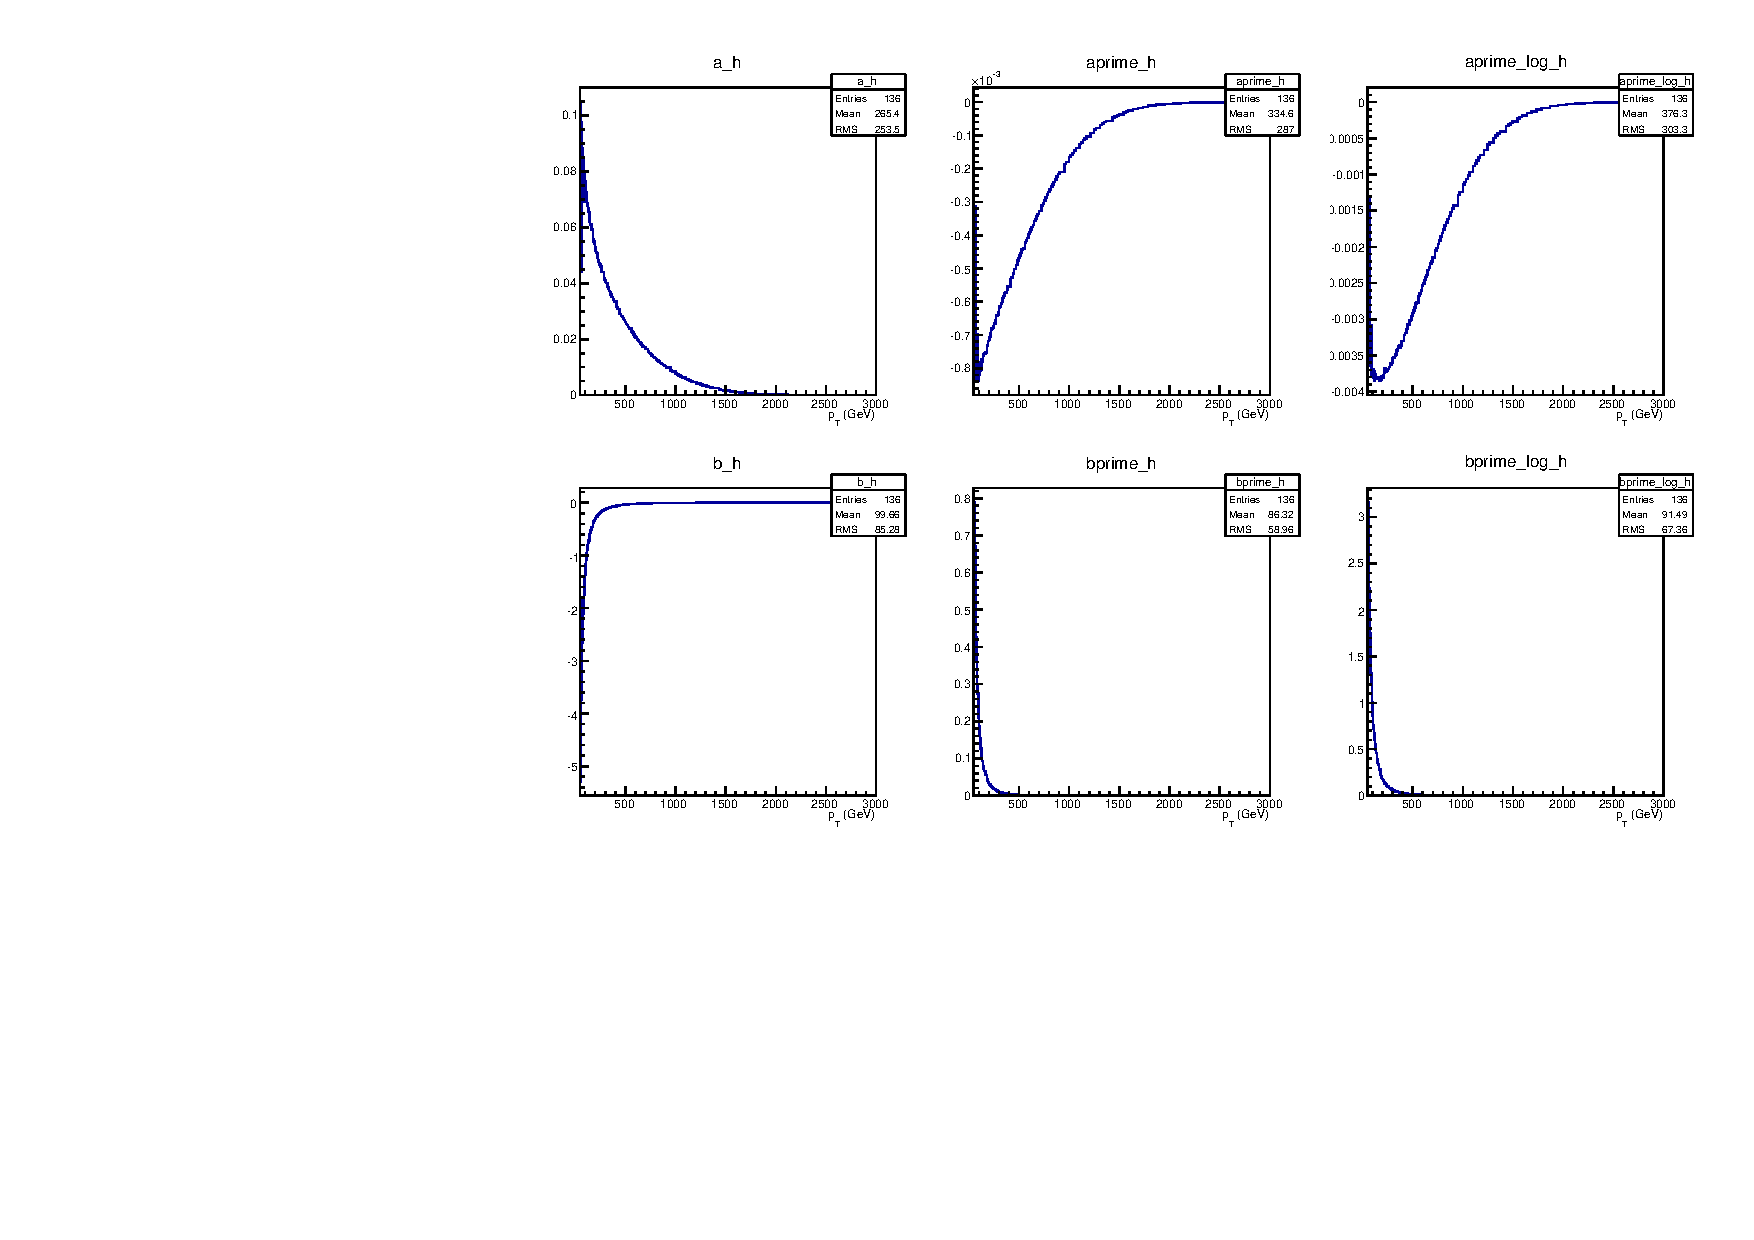
\includegraphics [width=0.9\linewidth] {central_coeffs_LL.pdf}
 \vspace {0.05 in}
\caption{}
\end{center}
\end{*figure} 
\end{frame}

\begin{frame}
\begin{*figure}
\begin{center}
 \vspace {0.05 in}
 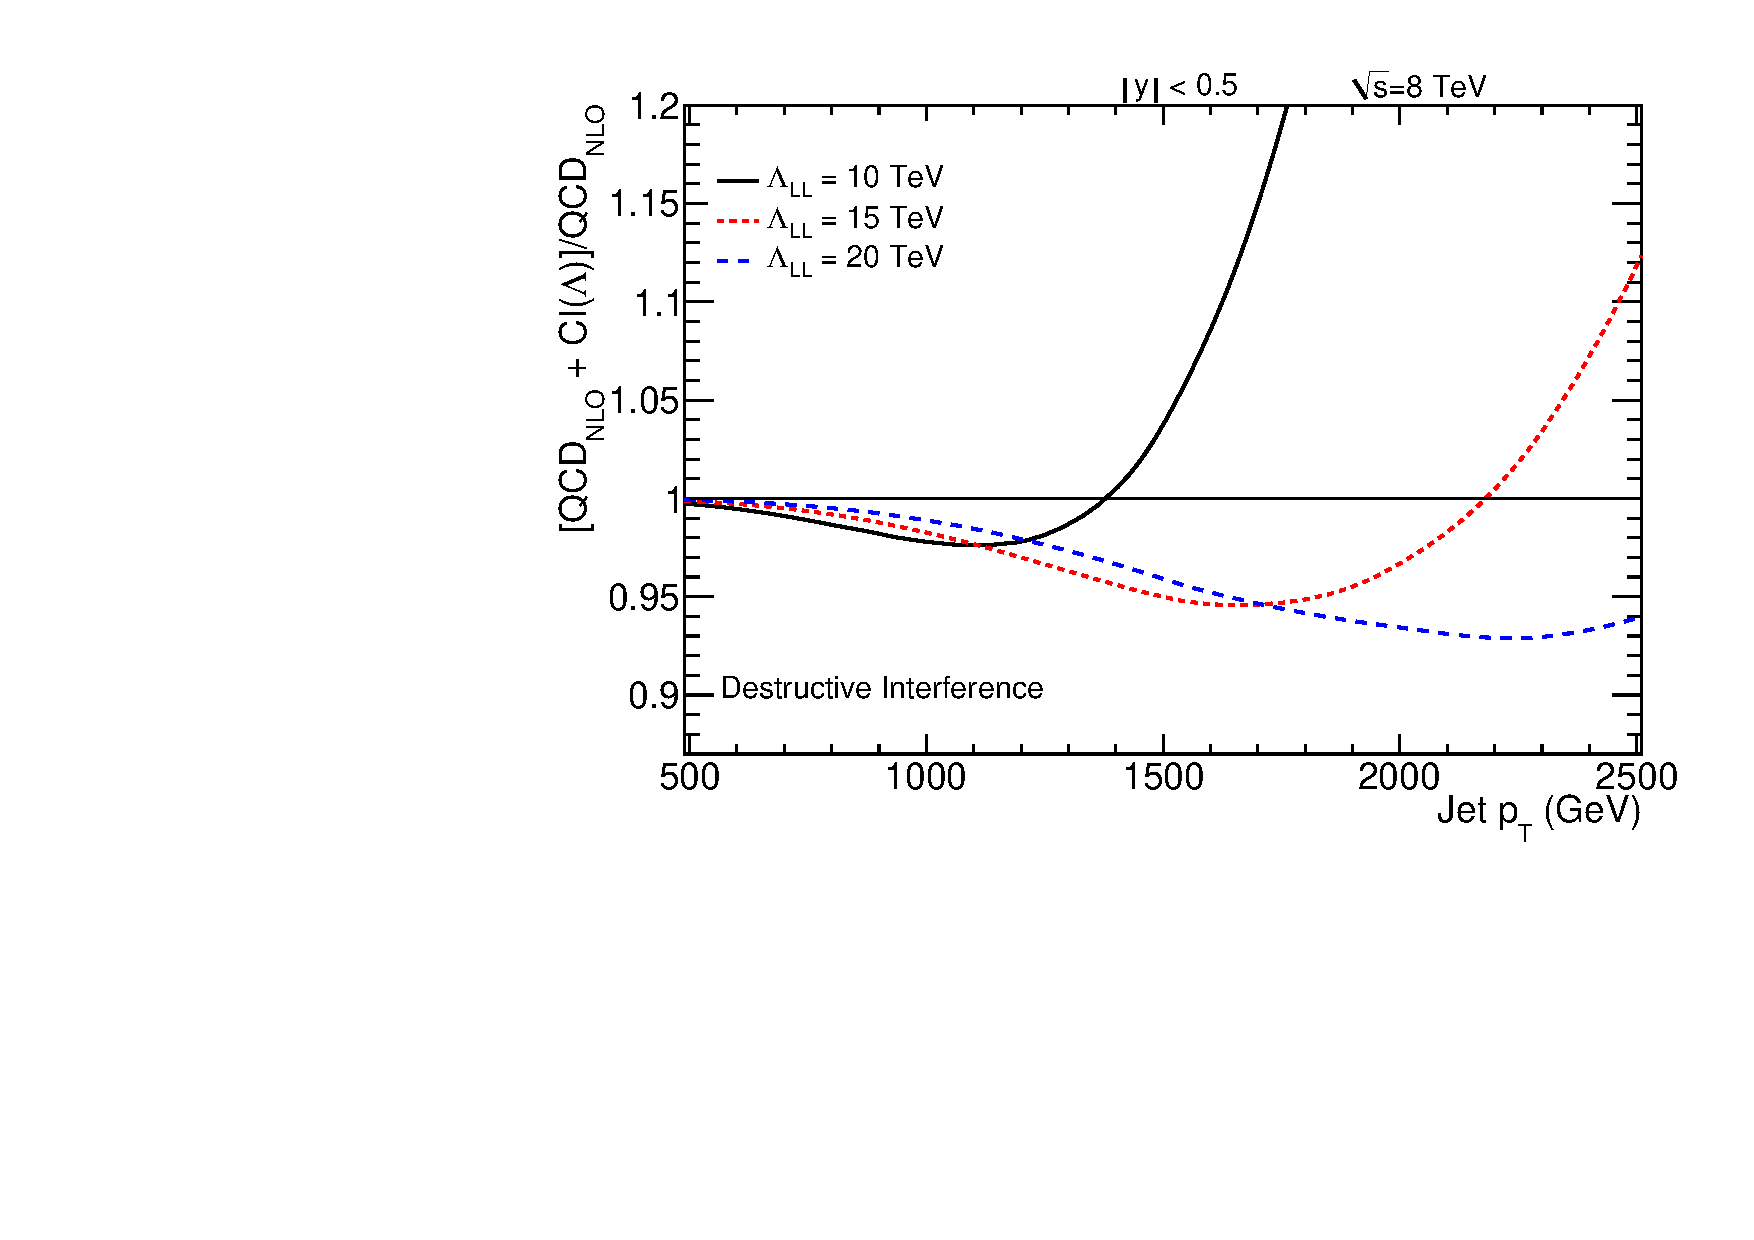
\includegraphics [width=0.9\linewidth] {LL_D.pdf}
 \vspace {0.05 in}
\caption{}
\end{center}
\end{*figure} 
\end{frame}

\begin{frame}
	\frametitle{Only PDF Uncertainty}
	\begin{*figure}
\begin{center}
 \vspace {0.05 in}
 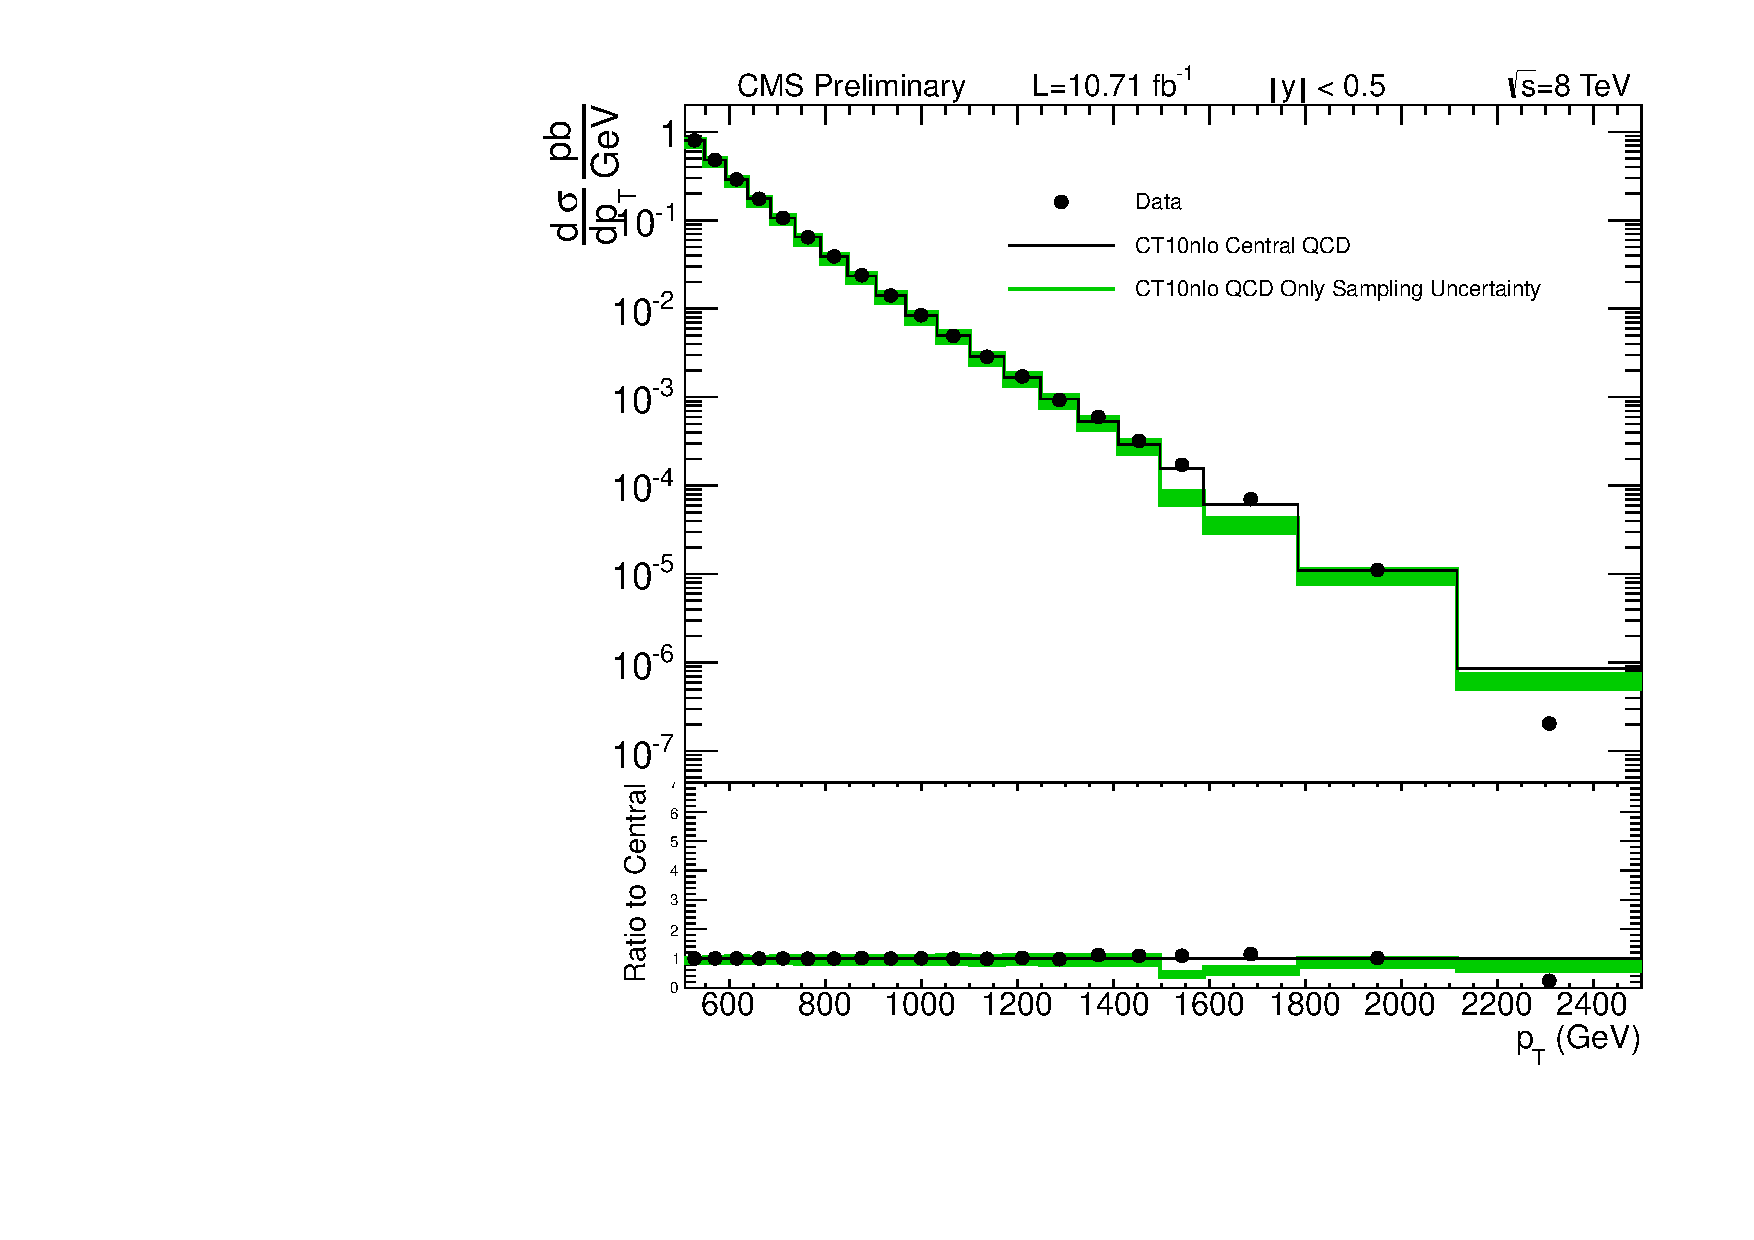
\includegraphics [width=0.7\linewidth] {xsec_CT10nlo_QCD_only_sampling.pdf}
 \vspace {0.05 in}
\caption{}
\end{center}
\end{*figure} 
\end{frame}

\begin{frame}
	\frametitle{Jet Smearing and PDF Uncertainty}
	\begin{*figure}
\begin{center}
 \vspace {0.05 in}
 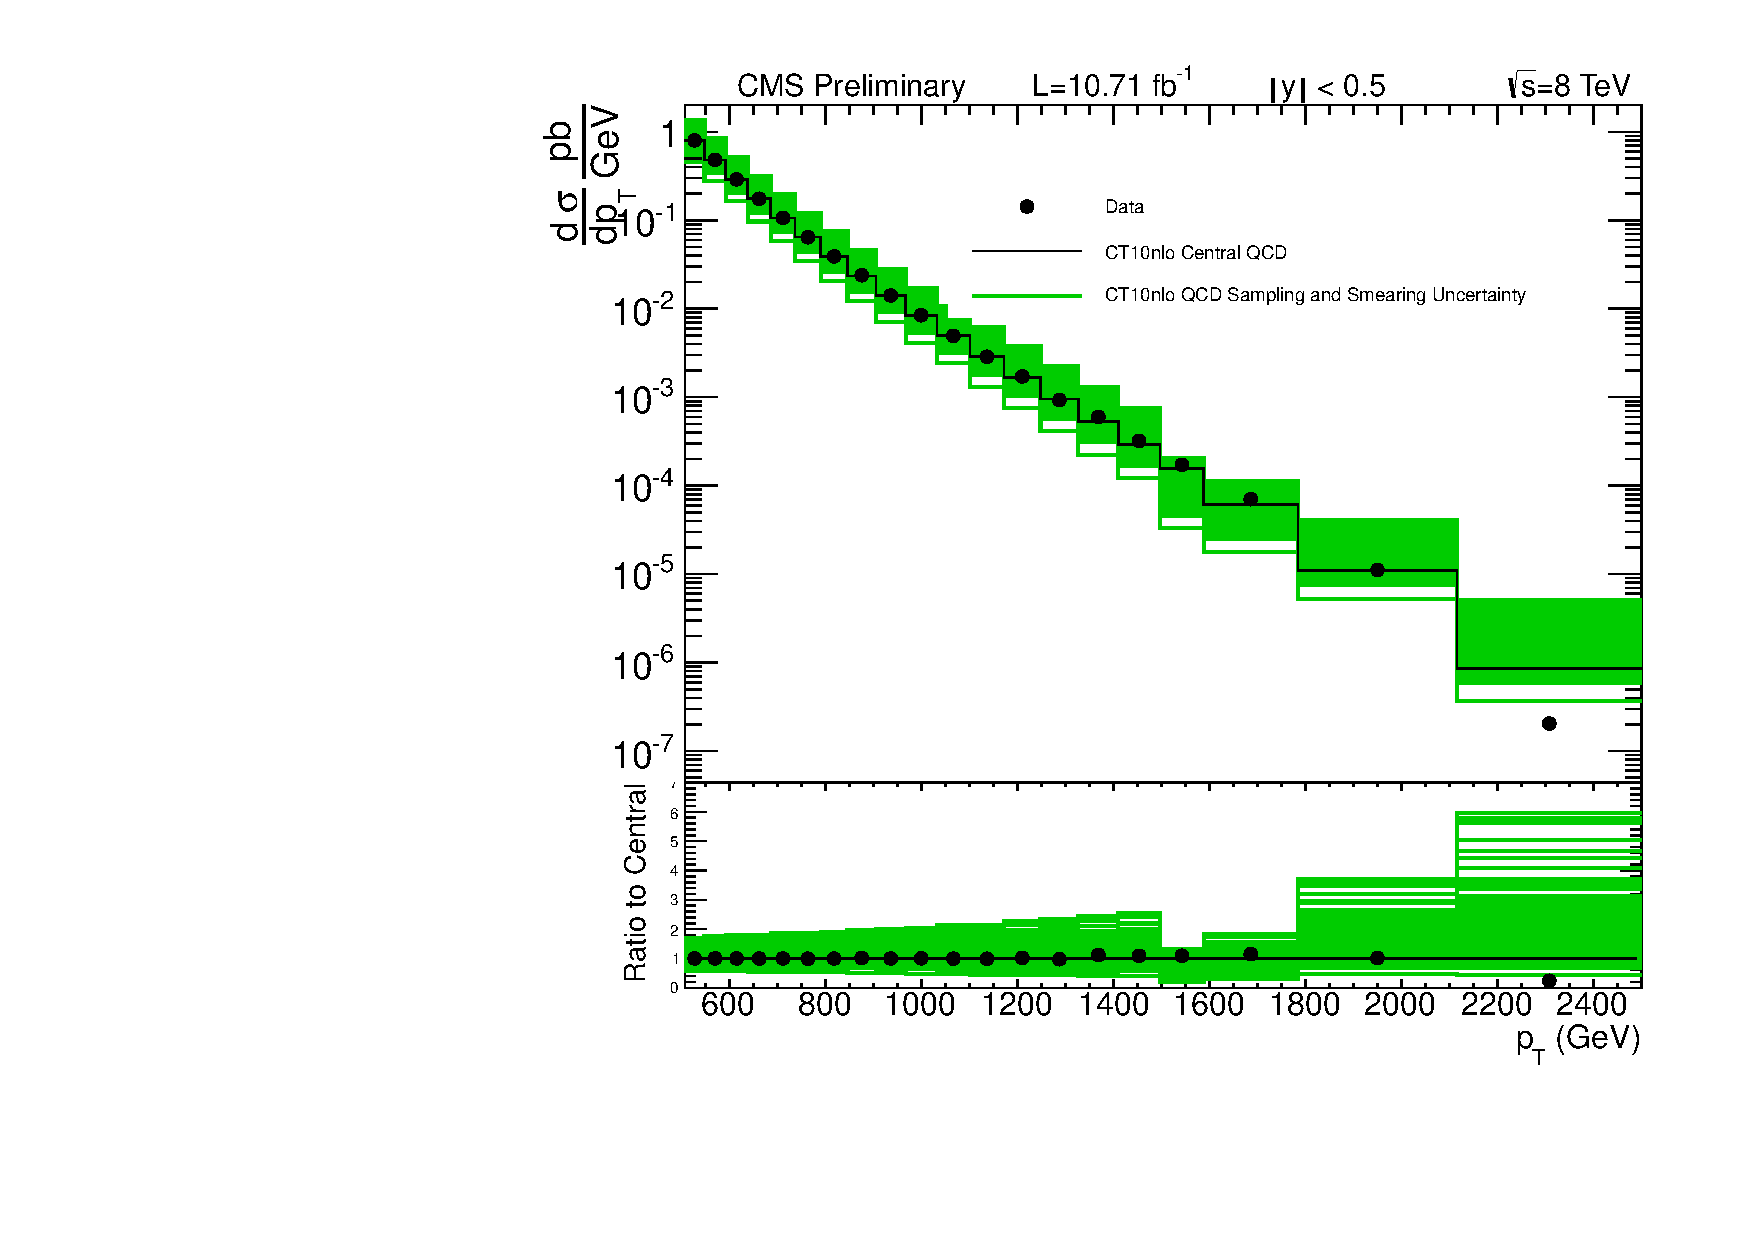
\includegraphics [width=0.7\linewidth] {xsec_CT10_QCD_sampled_and_smeared.pdf}
 \vspace {0.05 in}
\caption{ }
\end{center}
\end{*figure} 
\end{frame}

\begin{frame}
	\frametitle{Only PDF Uncertainty}
	\begin{*figure}
\begin{center}
 \vspace {0.05 in}
 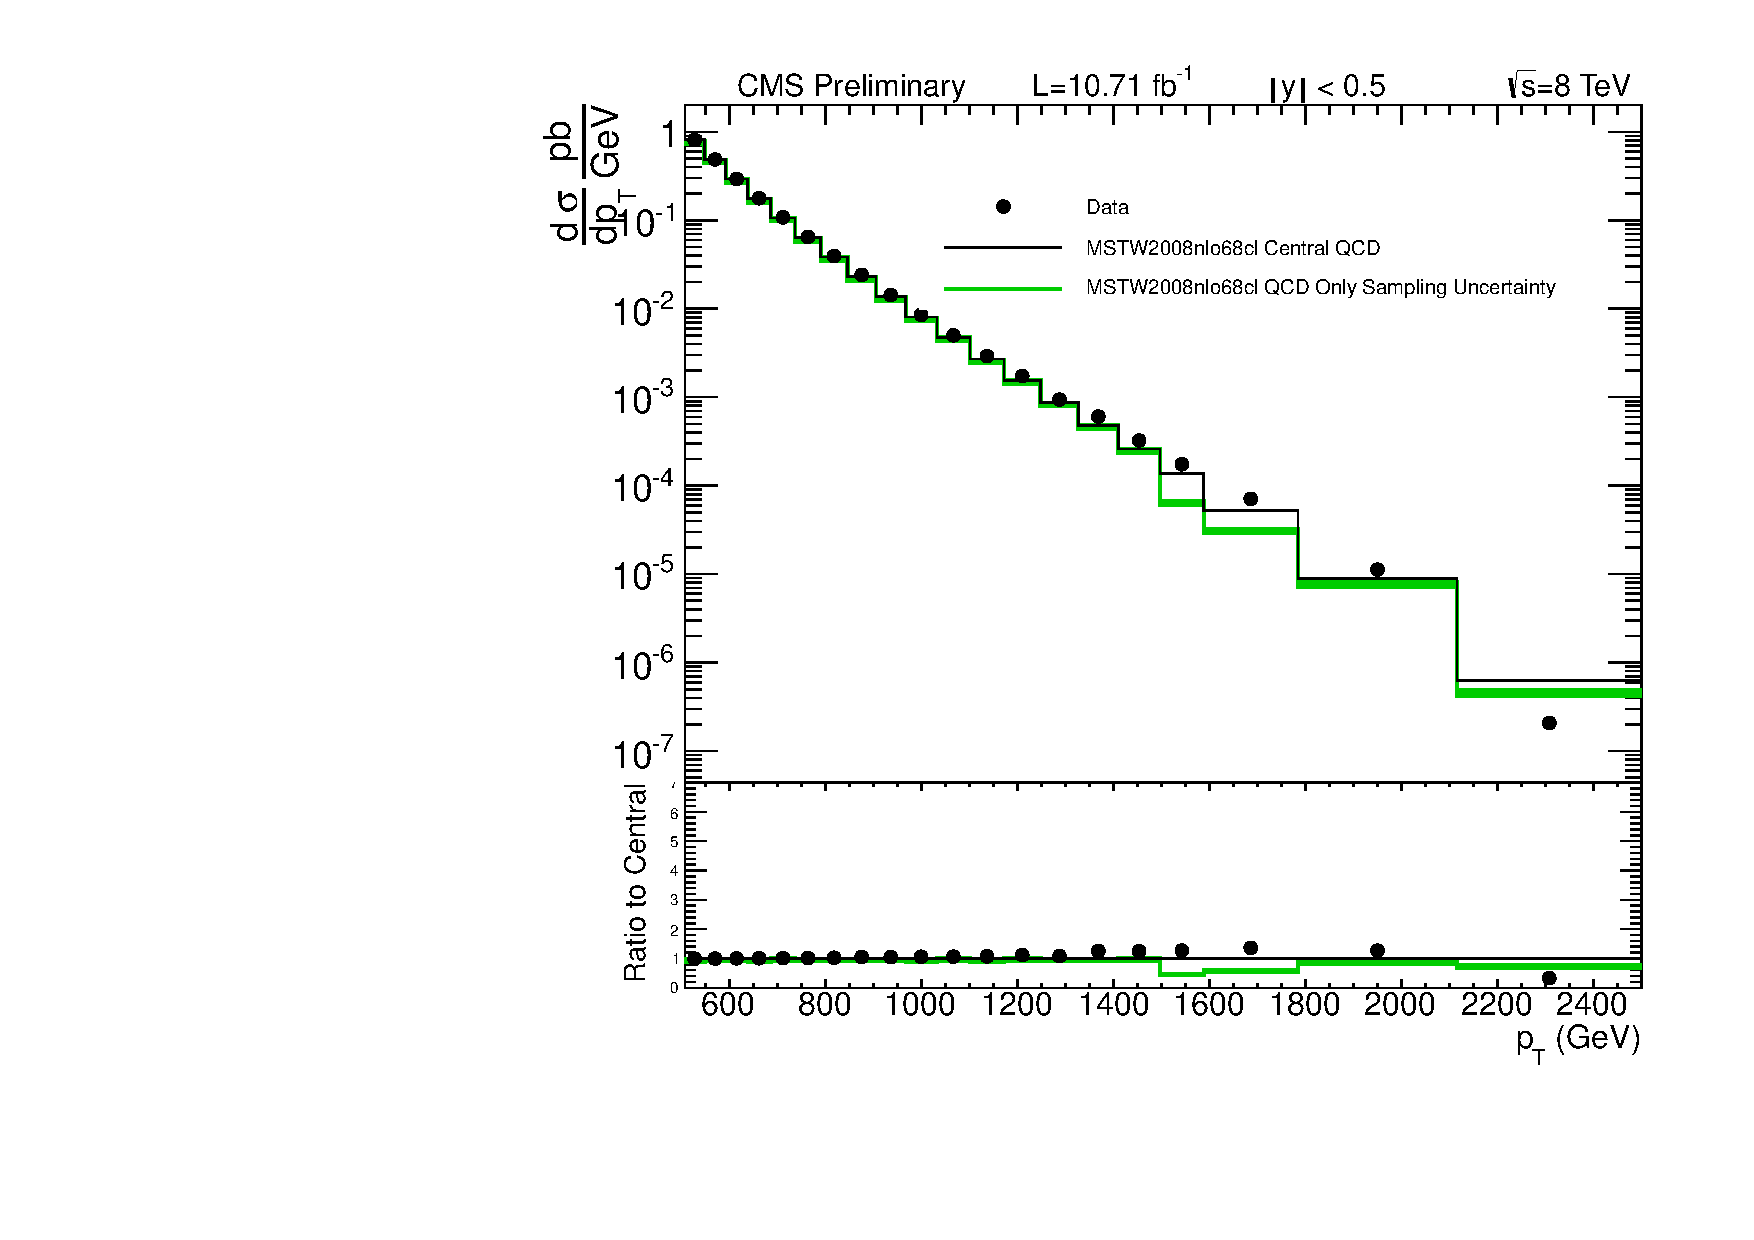
\includegraphics [width=0.7\linewidth] {xsec_MSTW_QCD_only_sampling.pdf}
 \vspace {0.05 in}
\caption{}
\end{center}
\end{*figure} 
\end{frame}

\begin{frame}
	\frametitle{Jet Smearing and PDF Uncertainty}
	\begin{*figure}
\begin{center}
 \vspace {0.05 in}
 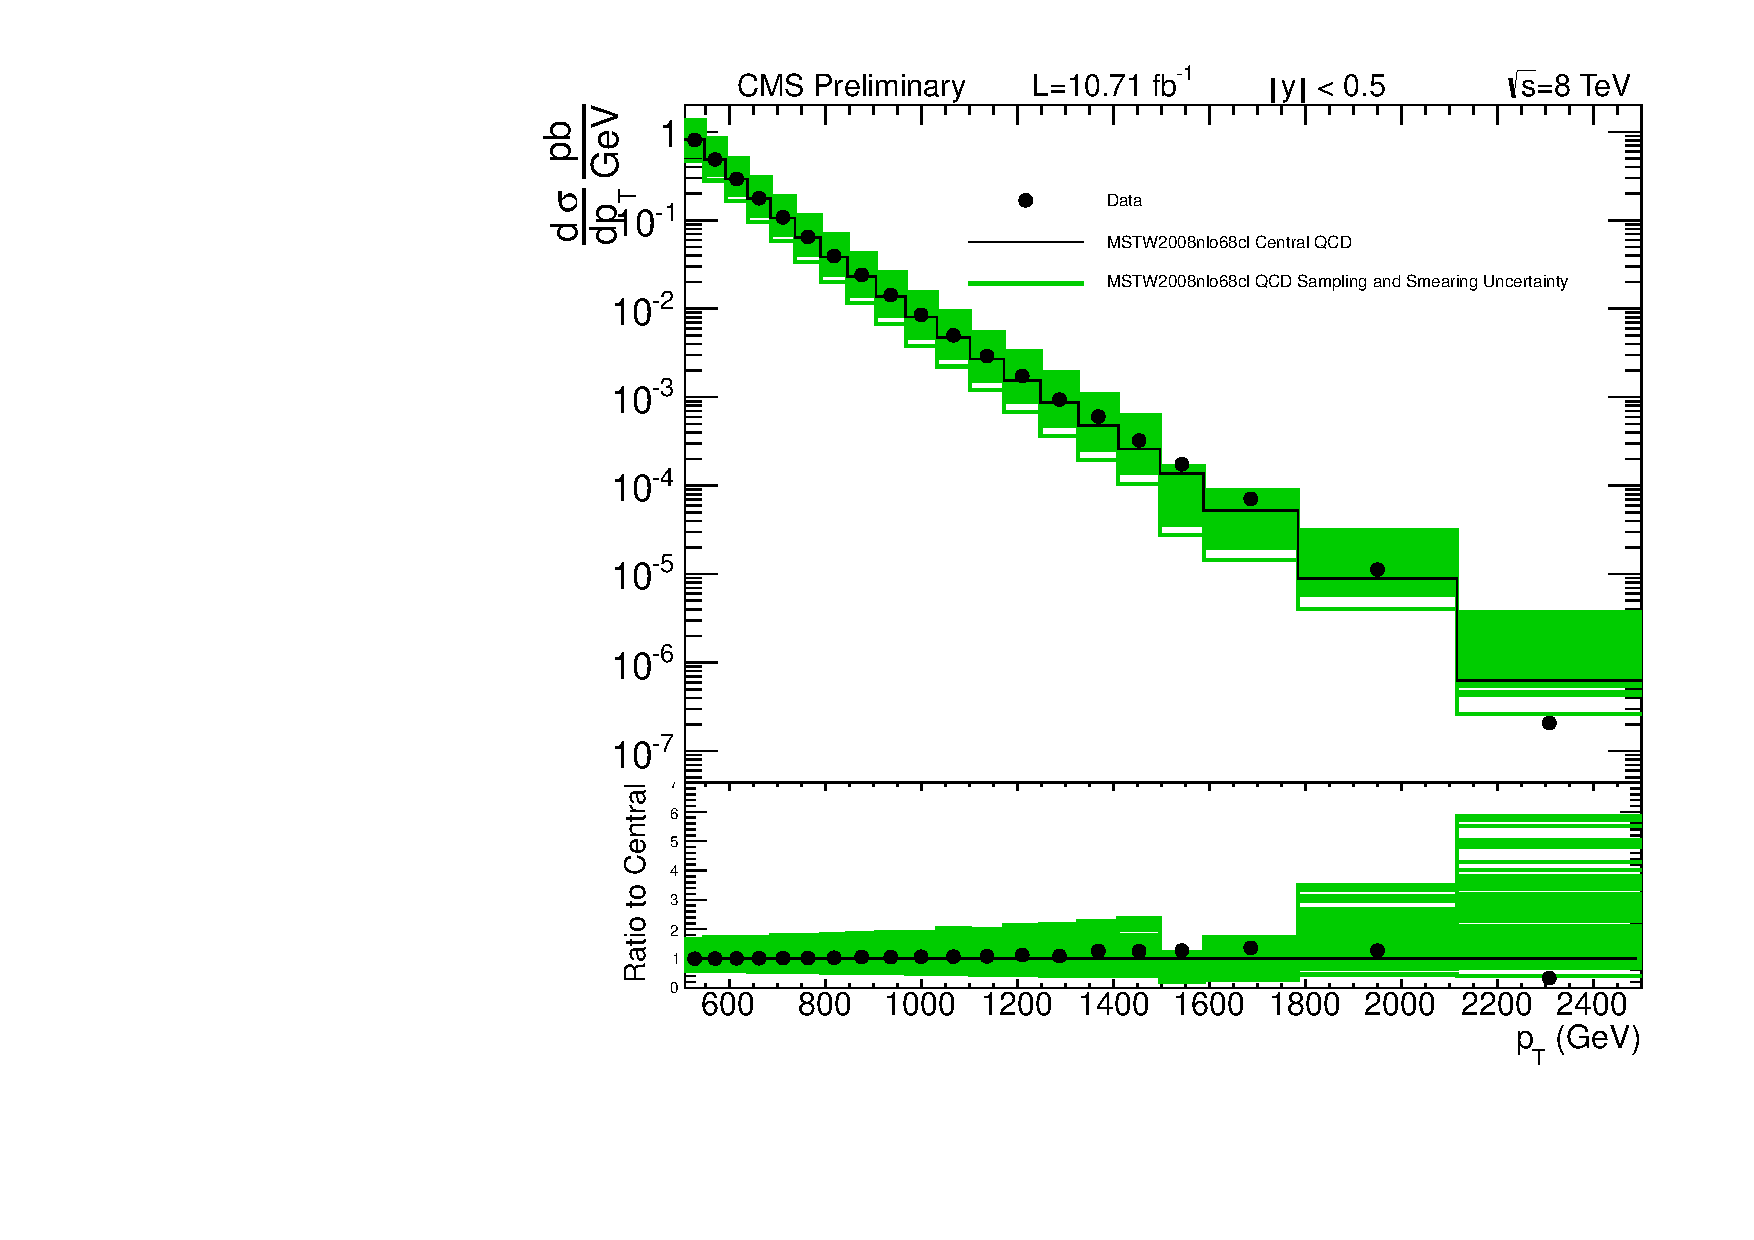
\includegraphics [width=0.7\linewidth] {xsec_MSTW_QCD_sampled_and_smeared.pdf}
 \vspace {0.05 in}
\caption{ }
\end{center}
\end{*figure} 
\end{frame}

\begin{frame}
	\frametitle{CI  withPDF Uncertainty}
	\begin{*figure}
\begin{center}
 \vspace {0.05 in}
 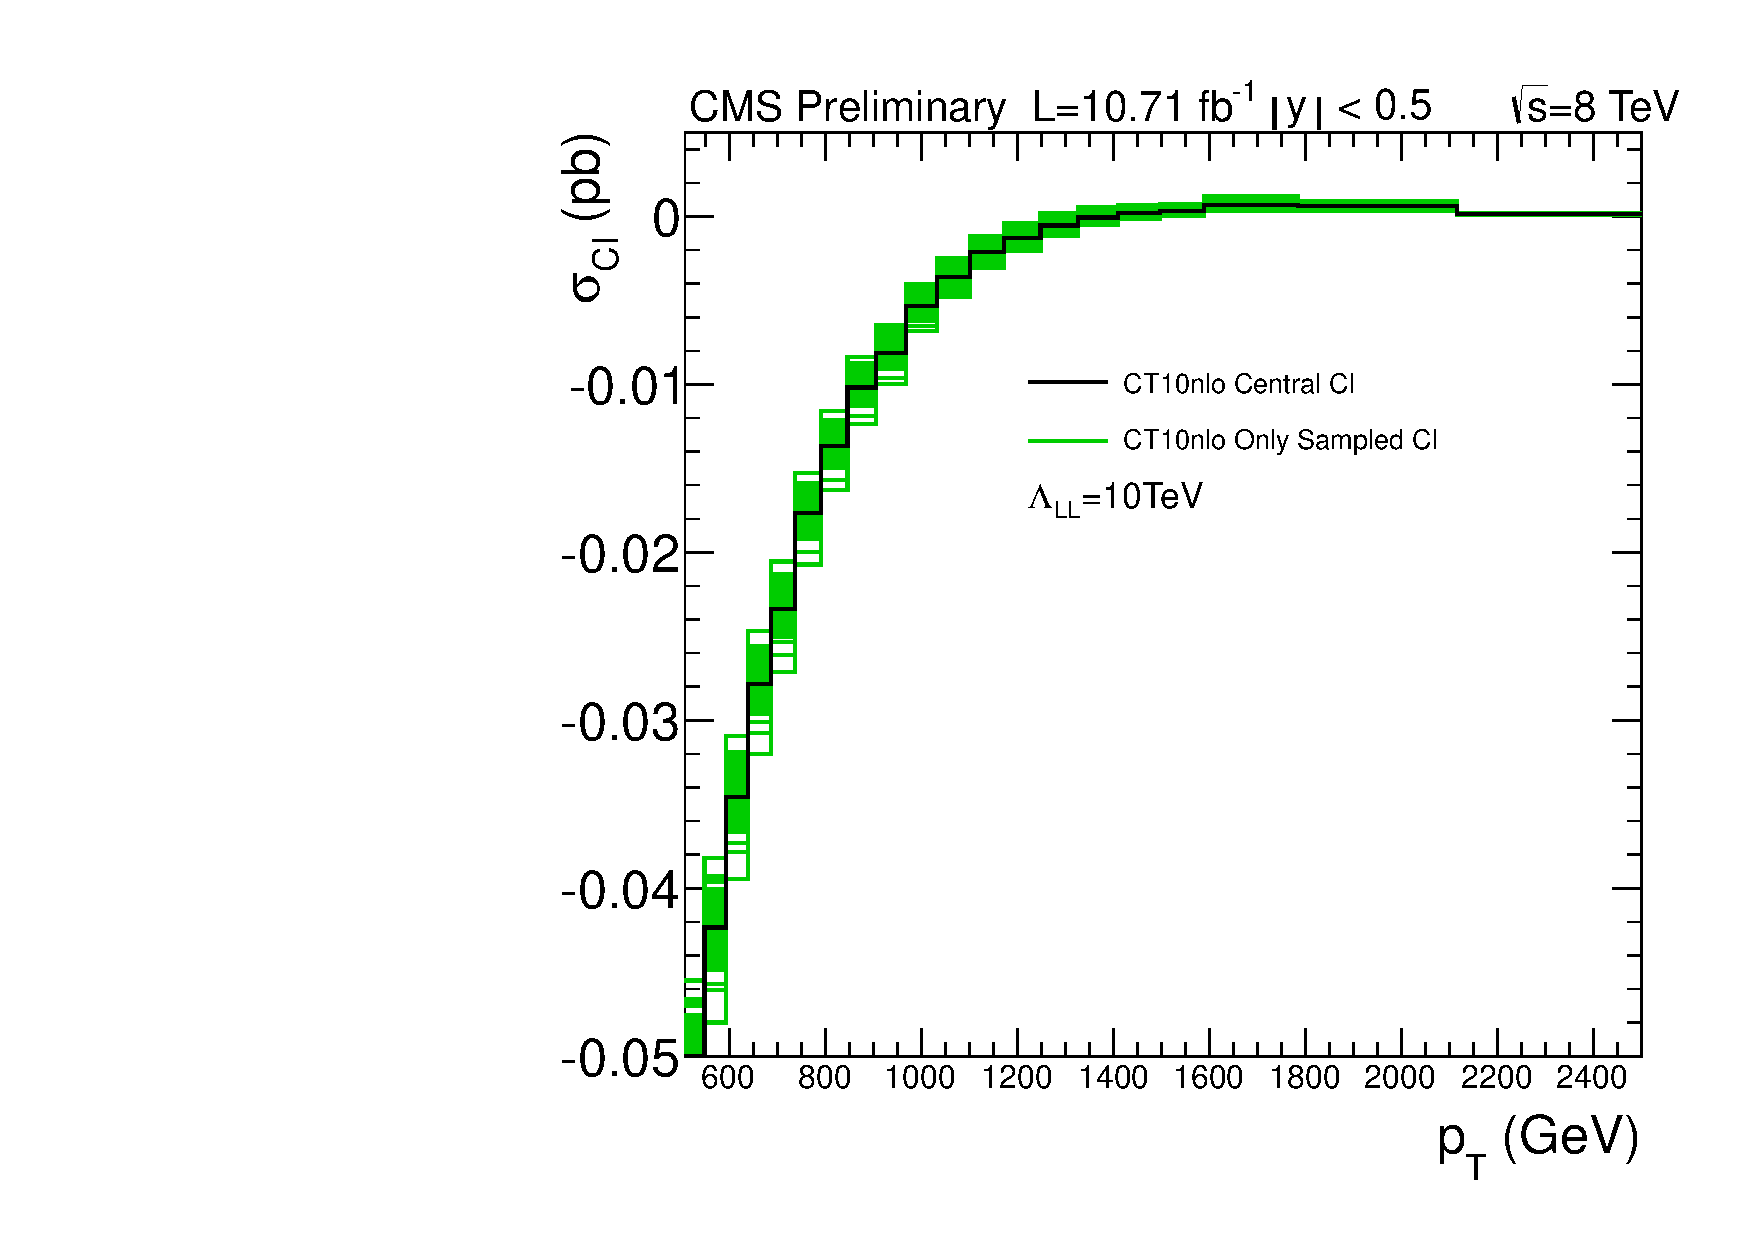
\includegraphics [width=0.7\linewidth] {10000_LL_sampled_xsec_CT10.pdf}
 \vspace {0.05 in}
\caption{ }
\end{center}
\end{*figure} 
\end{frame}

\begin{frame}
	\frametitle{CI  with PDF and Smearing Uncertainty}
	\begin{*figure}
\begin{center}
 \vspace {0.05 in}
 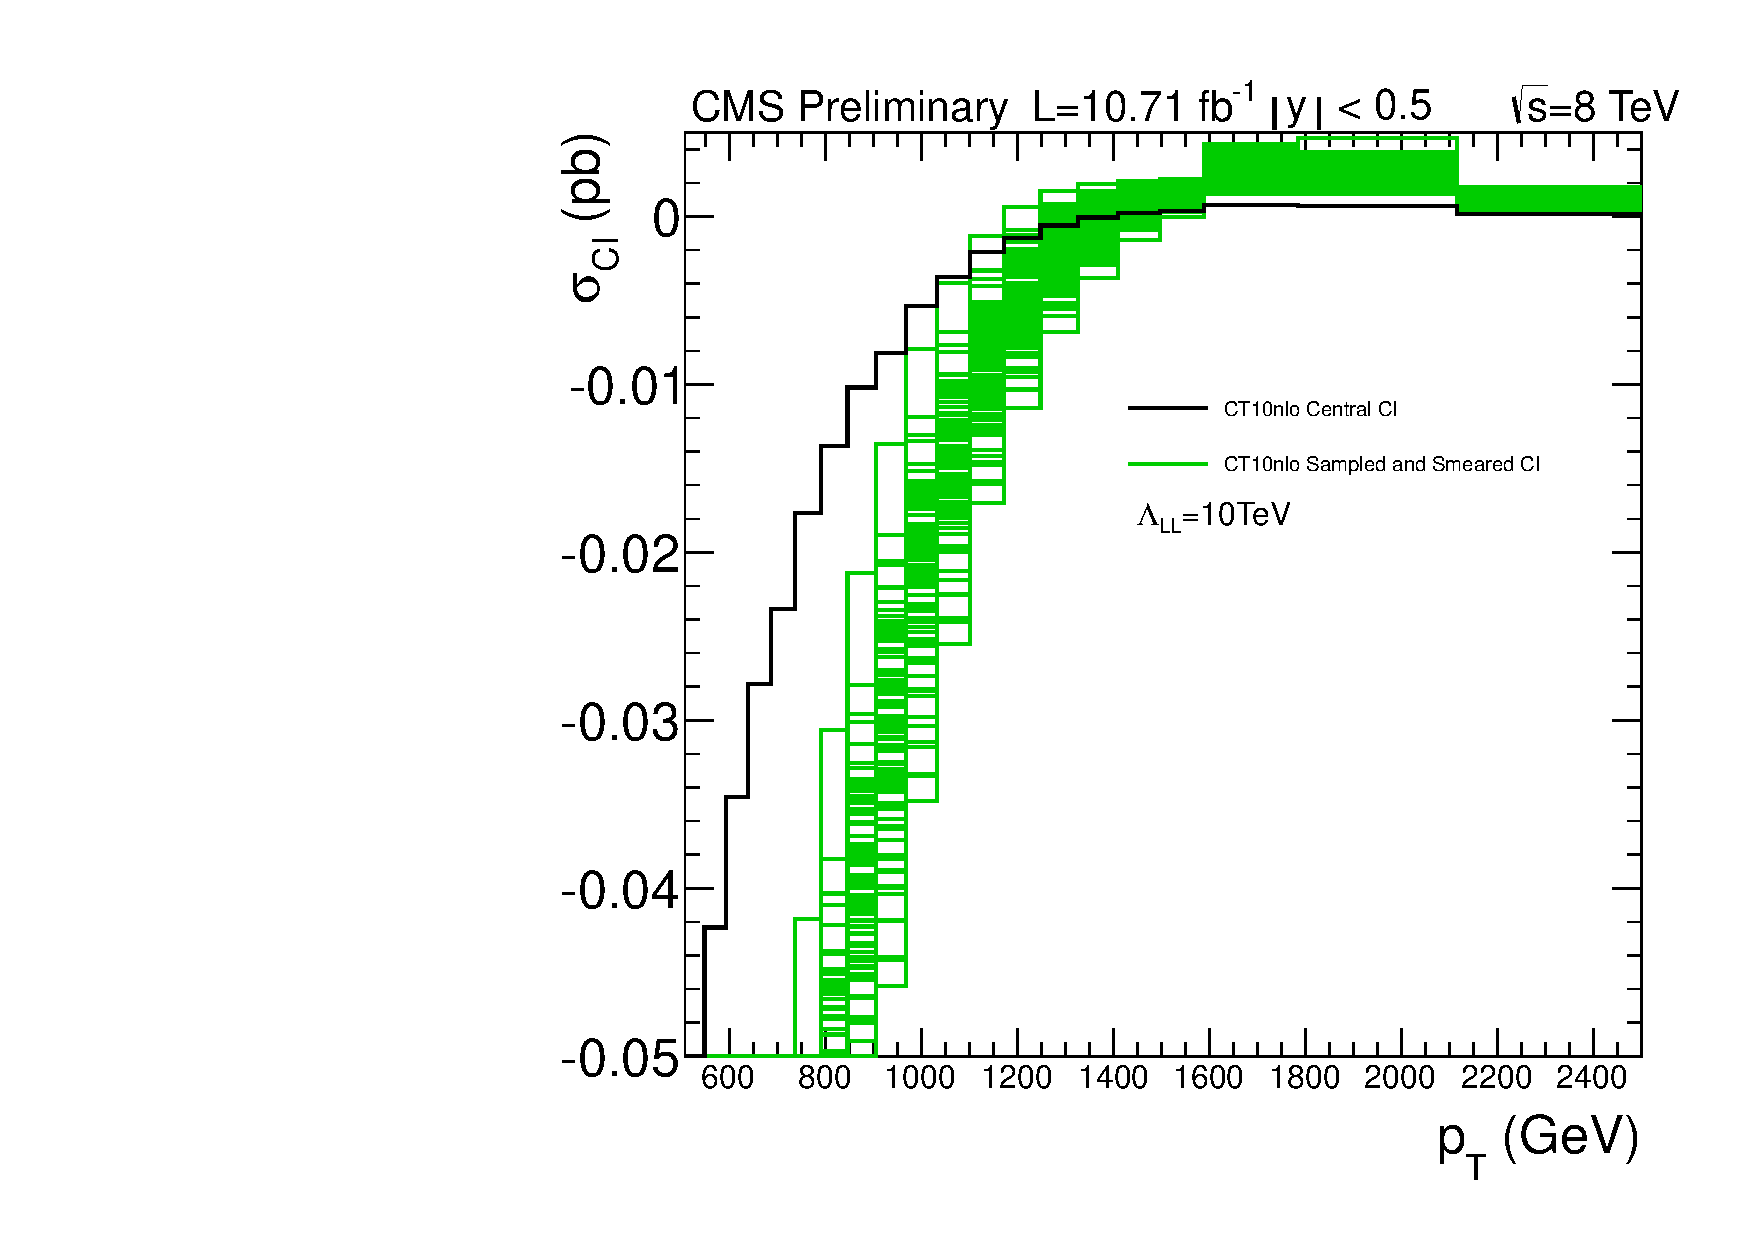
\includegraphics [width=0.7\linewidth] {10000_LL_sampled_and_smeared_xsec_CT10.pdf}
 \vspace {0.05 in}
\caption{ }
\end{center}
\end{*figure} 
\end{frame}

\begin{frame}
	\frametitle{To Do:}
	\begin{itemize}
		\item Sort out CI smearing issues
		\item Include PDF+Smearing Uncertainties on signal
		\item Compute limits on $\Lambda$ for each PDF and CI model
		\item Pool results from CT10nlo, MSTW2008nlo68cl, and NNPDF21\_100 PDF sets
		\item Currently drafting an analysis note
	\end{itemize}
\end{frame}

\end{document}